\documentclass[conference]{IEEEtran}

\usepackage{cite}
\usepackage{amsmath,amssymb,amsfonts}
\usepackage{algorithmic}
\usepackage{graphicx}
\usepackage{textcomp}
\usepackage{xcolor}
\usepackage{booktabs}
\usepackage{multirow}
\usepackage{url}
\usepackage{animate}

% Compile from the `paper/` directory so figures resolve via these paths.
\graphicspath{{../evaluation/plots/}{../evaluation/plots/explain/}{../evaluation/plots/explain/prop_frames/}}

\begin{document}

\title{Temporal Explainable GNN for Real-Time Intrusion Detection on Dynamic Network Graphs}

\author{%
\IEEEauthorblockN{Anonymous Author(s)}
\IEEEauthorblockA{%
This manuscript is prepared in IEEE conference format and can be updated with final author metadata before submission.}
}

\maketitle

\begin{abstract}
Network intrusion detection systems still struggle with two practical constraints: temporal behavior changes quickly, and operators need explanations they can trust. This work presents a temporal, explainable graph neural network (GNN) pipeline for real-time intrusion detection over dynamic flow graphs. We build snapshot graphs from CICIDS-style network flows, encode per-edge traffic features, and classify attack edges with a GAT-plus-LSTM model. To reduce evaluation optimism, preprocessing transforms are fitted on training data only and then frozen for validation and test. On the current project artifacts, our best upgraded temporal model reaches 0.904 F1 (recall 0.933, FAR 0.0319) at a detection-focused threshold, and 0.873 F1 (recall 0.841, FAR 0.0207) at a stricter low-false-alarm setting. We also report feature-level and attention-level explanations, plus replay-based real-time simulation, showing how the same model can be deployed in streaming mode with stable alert generation.
\end{abstract}

\begin{IEEEkeywords}
intrusion detection, graph neural network, temporal modeling, explainable AI, cybersecurity, real-time detection
\end{IEEEkeywords}

\section{Introduction}
Modern enterprise networks generate high-volume, high-velocity traffic where attack patterns evolve over time. Static classifiers over independent flows often miss these dynamics or produce brittle decisions under distribution shift. At the same time, operations teams need transparent alerts, not only scores.

This project addresses both issues by modeling traffic as temporal graph snapshots and adding explanation outputs during evaluation. The design objective is practical: one reproducible pipeline for training, offline evaluation, and near-real-time streaming inference.

The main contributions are:
\begin{itemize}
\item A reproducible temporal graph-learning pipeline with explicit leakage guards (train-only fitting for edge transforms and scaling).
\item A temporal edge-classification architecture combining graph attention and sequence modeling.
\item A deployment-ready inference path that tails live CSV flow streams and emits snapshot-level attack alerts.
\item Human-auditable explainability artifacts (feature permutation importance, attention traces, and gradient-based scores).
\end{itemize}

\section{Related Work}
Flow-based IDS research has moved from classical learners to deep sequence models and graph formulations. CICIDS2017-style benchmarks remain common for evaluating realistic attack diversity \cite{sharafaldin2018cicids}. Attention-based GNNs \cite{velickovic2018gat} are useful for heterogeneous connectivity patterns, while LSTMs \cite{hochreiter1997lstm} help capture temporal dependencies across windows. For imbalanced detection tasks, focal loss \cite{lin2017focal} is often used to focus learning on harder examples. Explainability in GNNs is an active area \cite{ying2019gnnexplainer}, especially for security use cases where operator trust is critical.

\section{Methodology}
\subsection{Traffic-to-Graph Construction}
Each flow record is assigned to a fixed-duration snapshot window (configured as 300 seconds). For every snapshot, source and destination endpoints form graph nodes, and each flow is an edge with seven traffic features:
\begin{itemize}
\item Flow Duration
\item Total Fwd Packets
\item Total Backward Packets
\item Total Length of Fwd Packets
\item Total Length of Bwd Packets
\item Flow Bytes/s
\item Flow Packets/s
\end{itemize}
Binary labels follow benign vs. attack semantics from the original flow label field.

To represent nodes, we compute lightweight structural and traffic summaries inside each snapshot: mean outgoing and incoming edge-feature vectors per endpoint, plus a normalized log connection-count feature. This yields node features that help the model distinguish ``busy'' servers, scans, and bursty communication patterns without requiring payload inspection.

\subsection{Temporal Explainable GNN}
Given snapshot sequence $\{\mathcal{G}_t\}_{t=1}^{T}$, node embeddings are computed by stacked graph attention layers:
\begin{equation}
\mathbf{H}_t^{(l+1)} = \mathrm{GAT}^{(l)}(\mathbf{H}_t^{(l)}, \mathbf{A}_t).
\end{equation}
Edge representations concatenate source/destination node embeddings with edge attributes, then pass through an edge MLP. A graph-level context vector per snapshot is built via mean pooling over edge embeddings and fed into an LSTM:
\begin{equation}
\mathbf{c}_{1:T} = \mathrm{LSTM}(\mathbf{g}_{1:T}).
\end{equation}
Final edge logits combine per-edge hidden states with time-aligned context states, then apply sigmoid for probabilities. Training uses focal BCE with class weighting to handle imbalance.

In our implementation, the backbone uses two GAT layers (first with multi-head attention, second with a single head), followed by an edge MLP. The temporal module runs an LSTM over the per-snapshot mean edge embedding (graph context), and each edge is classified using the concatenation of its edge embedding and the corresponding temporal context state.

\subsection{Leakage Guard and Split Policy}
To preserve deployment realism, clipping, log-transform, and standardization parameters are fitted only on the training split and reused unchanged for validation/test. Specifically, each edge feature is clipped to the 0.1\% and 99.9\% quantiles of the training split, transformed by $\log(1+x)$ (sign-aware for negative values), and finally standardized using a training-fitted scaler. The default split policy is \texttt{per\_day\_temporal} (70/15/15), with snapshot IDs disjoint across train/validation/test.

\subsection{Thresholding for Operating Modes}
Rather than fixing threshold at 0.5, threshold is selected from validation behavior to control false alarm rate (FAR) while maximizing F1/recall trade-offs. This supports multiple operating points (detection-focused vs. conservative SOC mode).

\section{Experimental Setup}
\subsection{Dataset and Scale}
Experiments use CICIDS2017 day-wise CSV captures (Monday through Friday attack scenarios), including DDoS, PortScan, Web Attacks, and Infiltration traffic \cite{sharafaldin2018cicids}. Current project statistics show 1,559,907 flow rows in the processed dataset summary.

\subsection{Training Configuration}
Core settings from \texttt{config.yml} include 40 epochs, early stopping patience 8, learning rate $8\times10^{-4}$ (with upgraded rank configuration exploring $5\times10^{-4}$), dropout 0.2, hidden dimension 64, and snapshot chunk size 4 for temporal context.

\subsection{Baselines and Metrics}
Reported metrics include accuracy, precision, recall, F1, ROC-AUC, FAR, and detection rate (DR). The available model comparison artifact reports the upgraded temporal model against a stacked logistic meta-learner baseline.

\section{Results and Discussion}
\subsection{Primary Detection Performance}
Table~\ref{tab:modelcomp} shows that the upgraded temporal GNN outperforms the stacked baseline on F1 and recall while maintaining very low FAR.

\begin{table}[htbp]
\caption{Model Comparison (from \texttt{evaluation/model\_comparison.csv})}
\label{tab:modelcomp}
\centering
\begin{tabular}{lcccc}
\toprule
Model & Acc. & Prec. & Recall & F1 \\
\midrule
TemporalGNN\_Upgraded\_Rank1 & 0.9522 & 0.9080 & 0.8410 & 0.8732 \\
StackedMetaLR & 0.9496 & 0.9066 & 0.8279 & 0.8655 \\
\bottomrule
\end{tabular}
\end{table}

\subsection{Operating-Point Trade-off}
Two operating points are particularly useful for deployment:
\begin{itemize}
\item \textbf{Detection-focused} (threshold 0.8): F1 0.9039, recall 0.9328, FAR 0.0319.
\item \textbf{Conservative} (threshold 0.9): F1 0.8732, recall 0.8410, FAR 0.0207.
\end{itemize}
This gives teams a practical way to tune sensitivity vs. alert fatigue.

At the conservative operating point (threshold 0.9), the available confusion counts are TN=2456, FP=52, FN=97, and TP=513, which illustrates that FAR can be held low while still capturing a majority of attack edges.

\subsection{Hyperparameter Search Signal}
Large-grid HPO artifacts indicate the strongest validation F1 values are concentrated around hidden size 64 and single-head attention configurations, with recall frequently above 0.95 in top-ranked settings. This supports the final lightweight architecture choice.

\begin{figure}[htbp]
\centerline{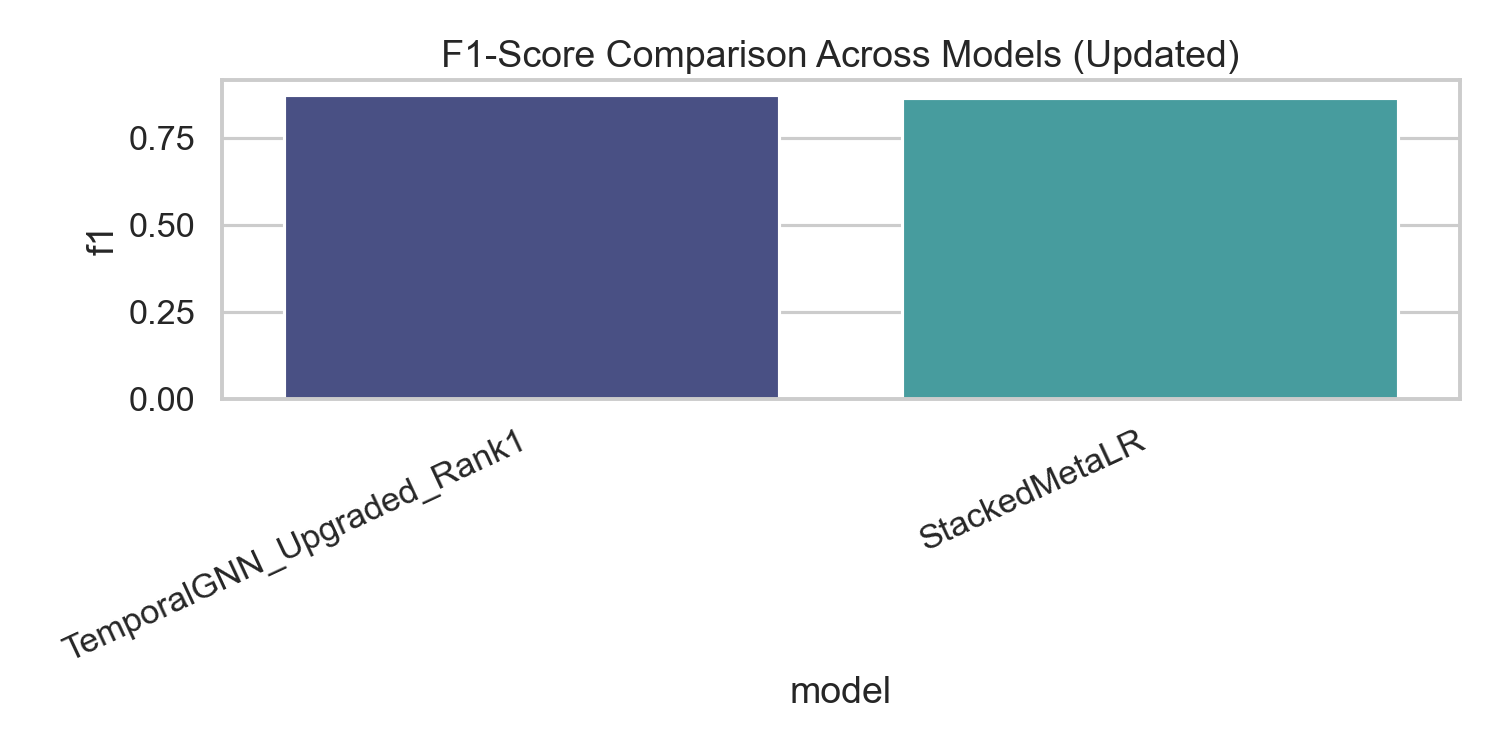
\includegraphics[width=0.95\columnwidth]{f1_model_comparison_updated.png}}
\caption{F1 comparison among available evaluated models.}
\label{fig:f1comp}
\end{figure}

\section{Explainability and Real-Time Behavior}
\subsection{Feature-Level Explanations}
Permutation analysis ranks packet-length and packet-count features as the dominant contributors. The top features are Total Length of Bwd Packets, Total Length of Fwd Packets, and Total Fwd Packets. This is consistent with attack traffic that often changes flow volume characteristics.

\begin{figure}[htbp]
\centerline{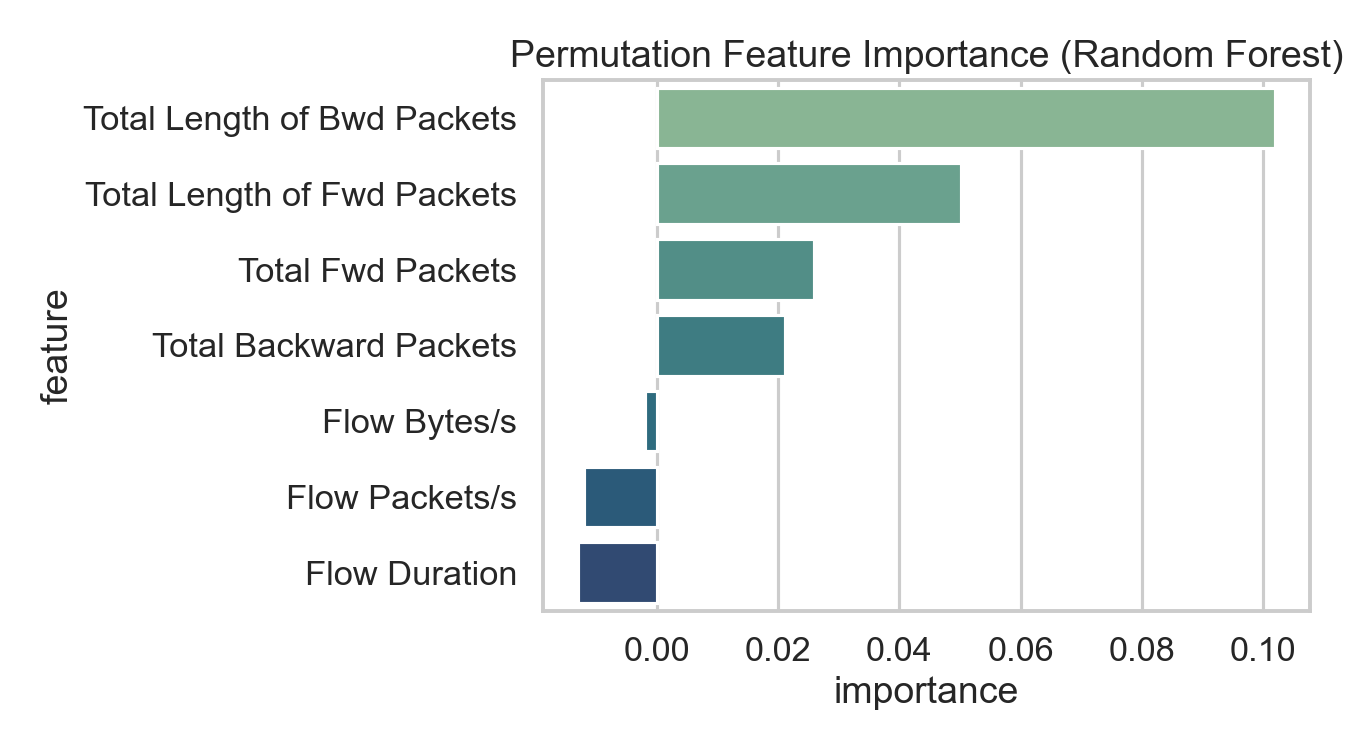
\includegraphics[width=0.95\columnwidth]{permutation_feature_importance.png}}
\caption{Permutation feature importance from explainability artifacts.}
\label{fig:perm}
\end{figure}

\subsection{Attention/Attribution Outputs}
Saved attention traces and gradient attribution snapshots (\texttt{evaluation/explain/} and \texttt{evaluation/plots/explain/}) provide localized evidence about which edges and attributes influenced decisions. While these are not causal proofs, they are useful for analyst triage and sanity checks.

Additional generated evaluation artifacts are included to help validate and inspect model behaviour. Figure~\ref{fig:rocpr} shows ROC and Precision-Recall curves for the final temporal model; Figure~\ref{fig:explain_examples} presents example attention and gradient-attribution visualizations for a detected snapshot. Full artifact sets (loss curves, confusion matrices, constructed graph visualizations, feature distributions, and additional explain plots) are available in the repository under \texttt{evaluation/plots/} and \texttt{evaluation/plots/explain/}.

\begin{figure}[htbp]
\centering
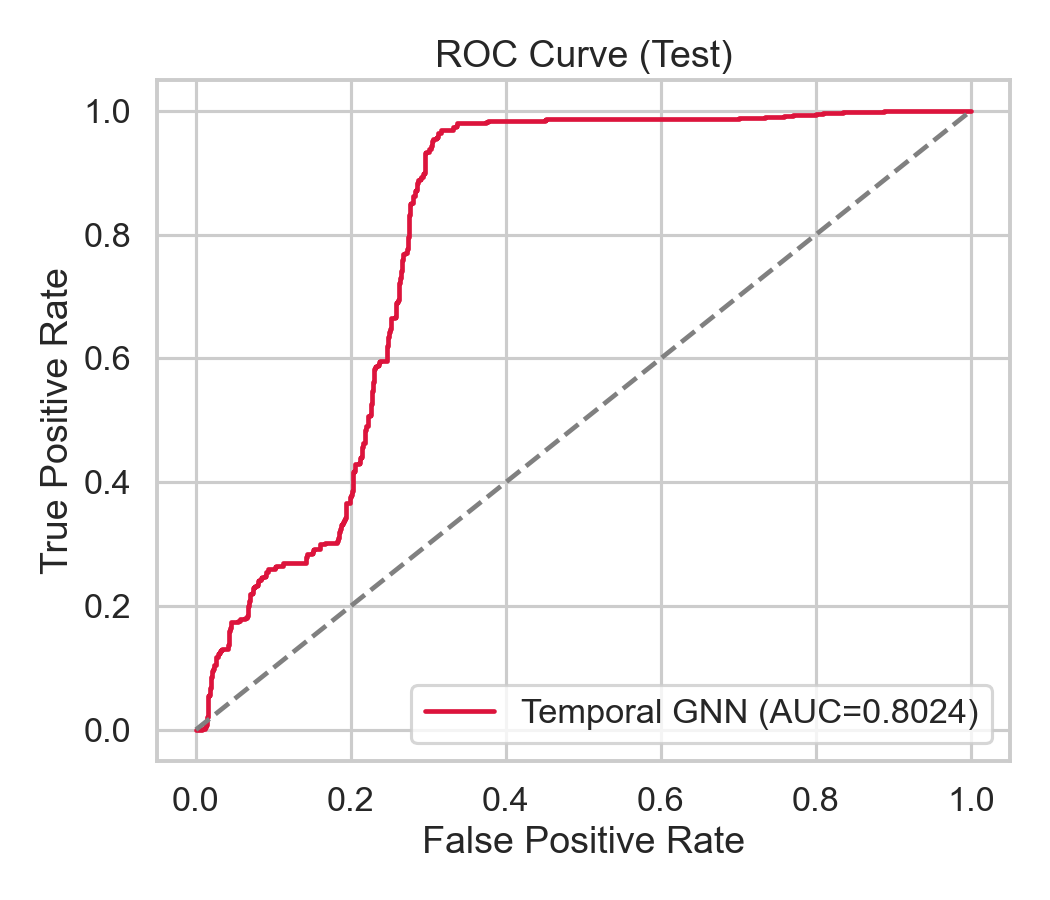
\includegraphics[width=0.48\columnwidth]{roc_temporal_gnn.png}
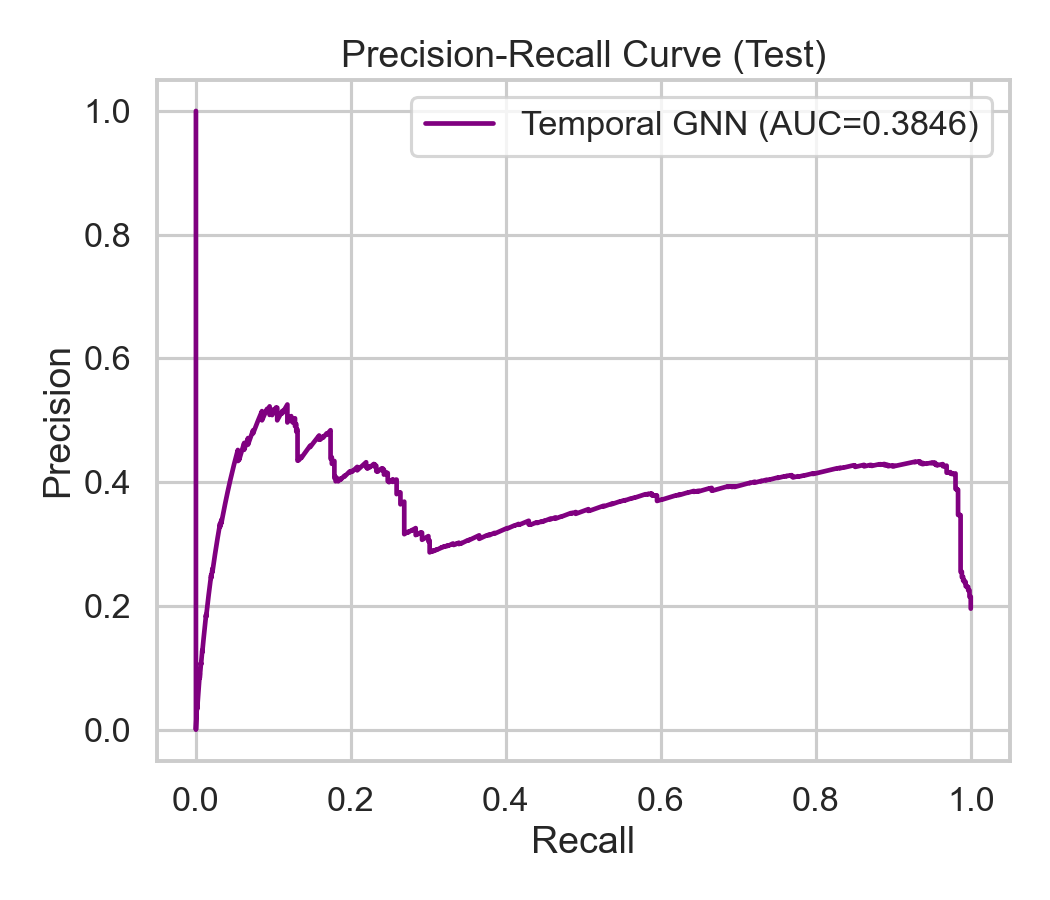
\includegraphics[width=0.48\columnwidth]{pr_temporal_gnn.png}
\caption{Receiver Operating Characteristic (left) and Precision-Recall (right) curves for the upgraded temporal GNN.}
\label{fig:rocpr}
\end{figure}

\begin{figure}[htbp]
\centering
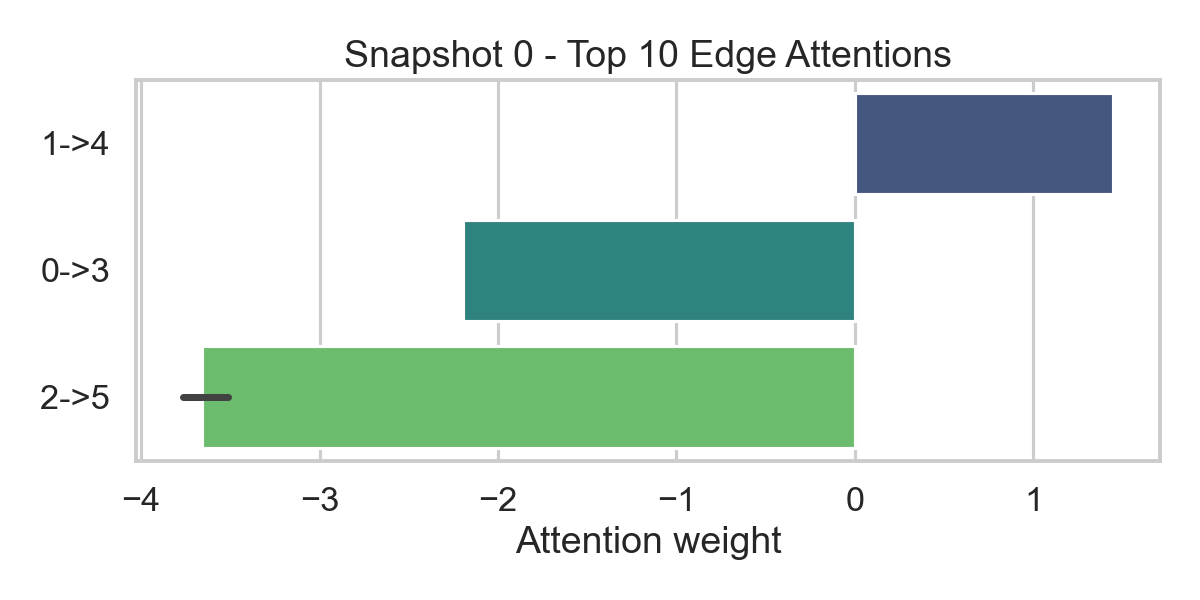
\includegraphics[width=0.48\columnwidth]{explain/attention_snapshot_0.png}
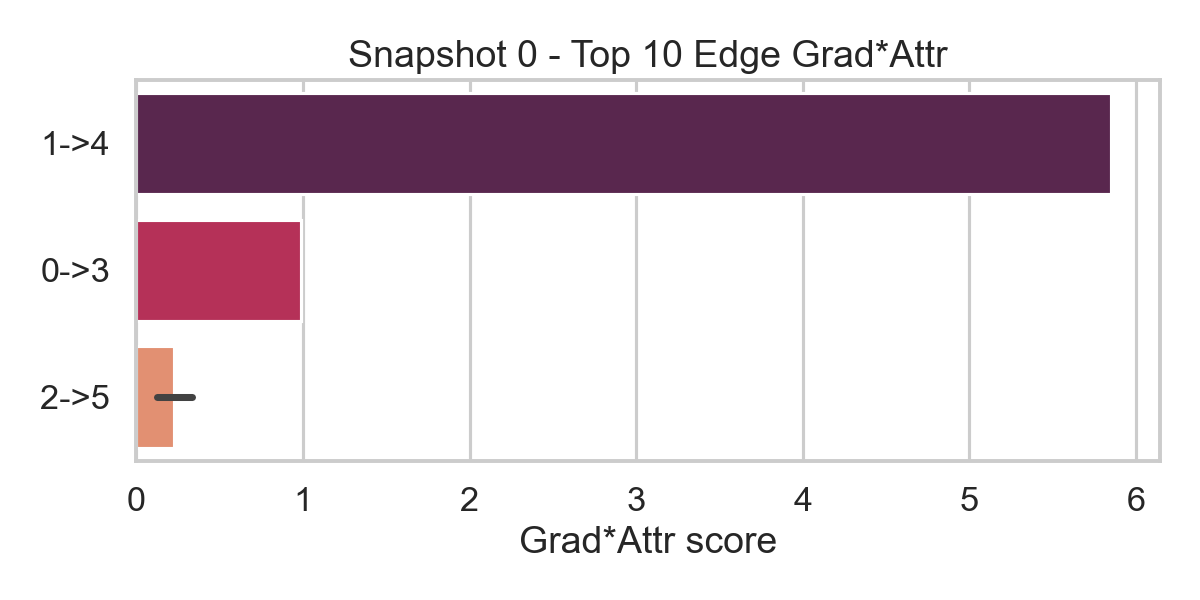
\includegraphics[width=0.48\columnwidth]{explain/grad_attr_snapshot_0.png}
\caption{Example explainability artifacts: attention heatmap (left) and gradient attribution overlay (right) for a high-confidence attack snapshot.}
\label{fig:explain_examples}
\end{figure}

\begin{figure}[htbp]
\centering
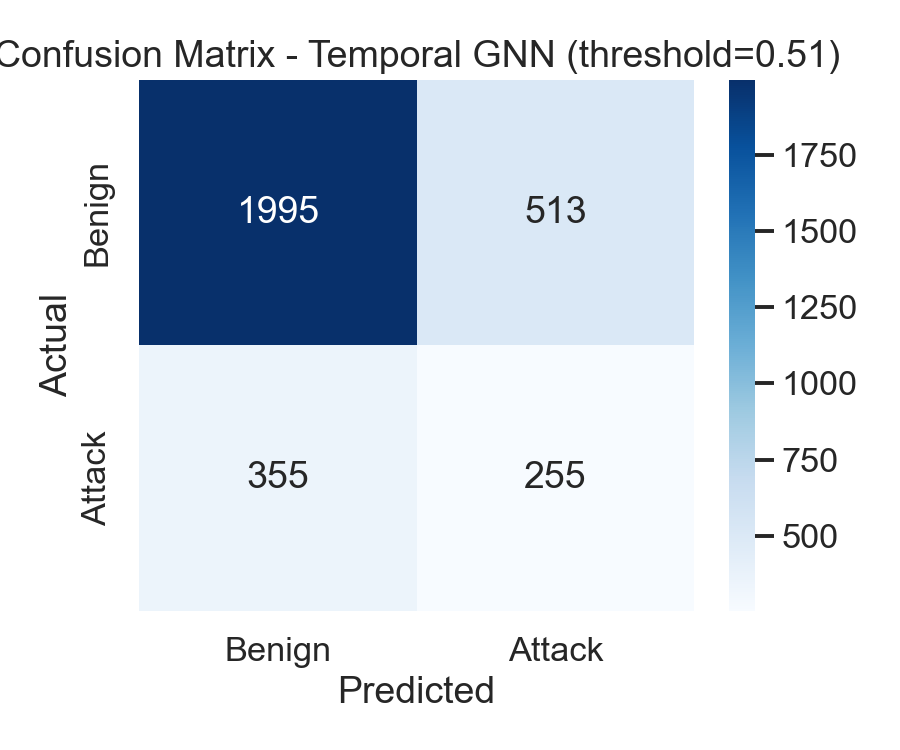
\includegraphics[width=0.48\columnwidth]{confusion_matrix_temporal_gnn.png}
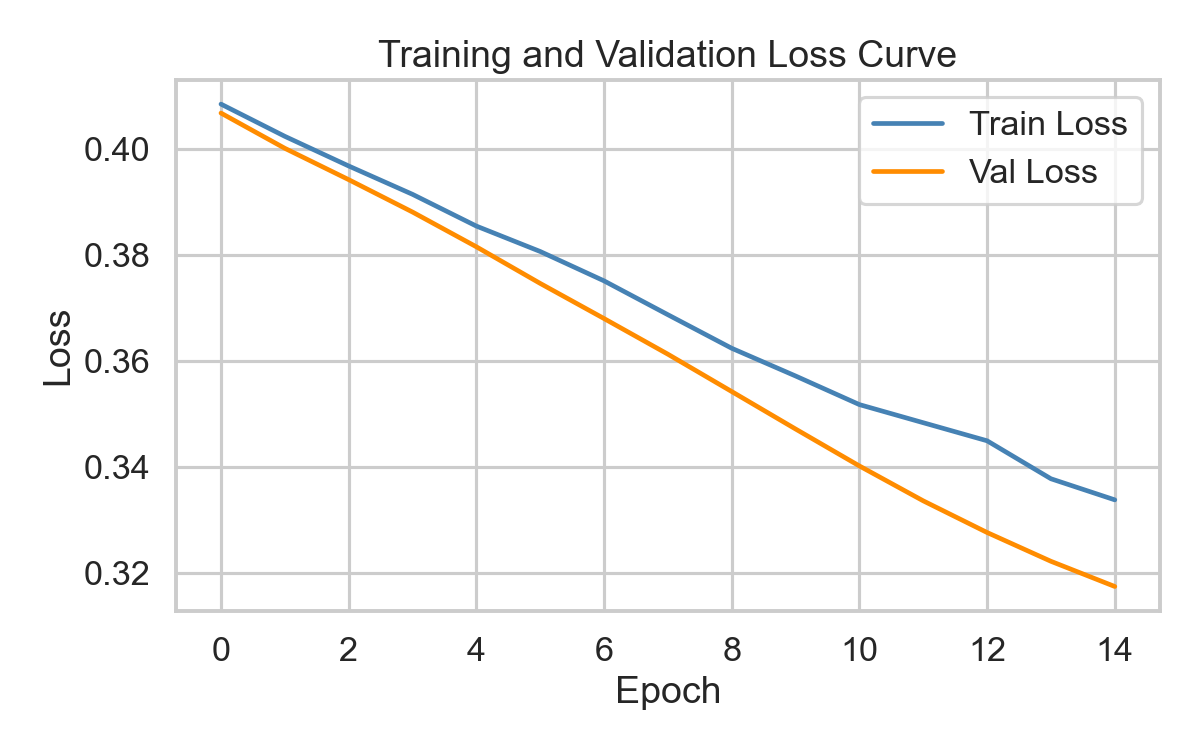
\includegraphics[width=0.48\columnwidth]{loss_curve_temporal_gnn.png}
\caption{Confusion matrix (left) and training loss curve (right) for the upgraded temporal GNN.}
\label{fig:conf_loss}
\end{figure}

\begin{figure}[htbp]
\centering
\includegraphics[width=0.32\columnwidth]{constructed_graph_snapshot.png}
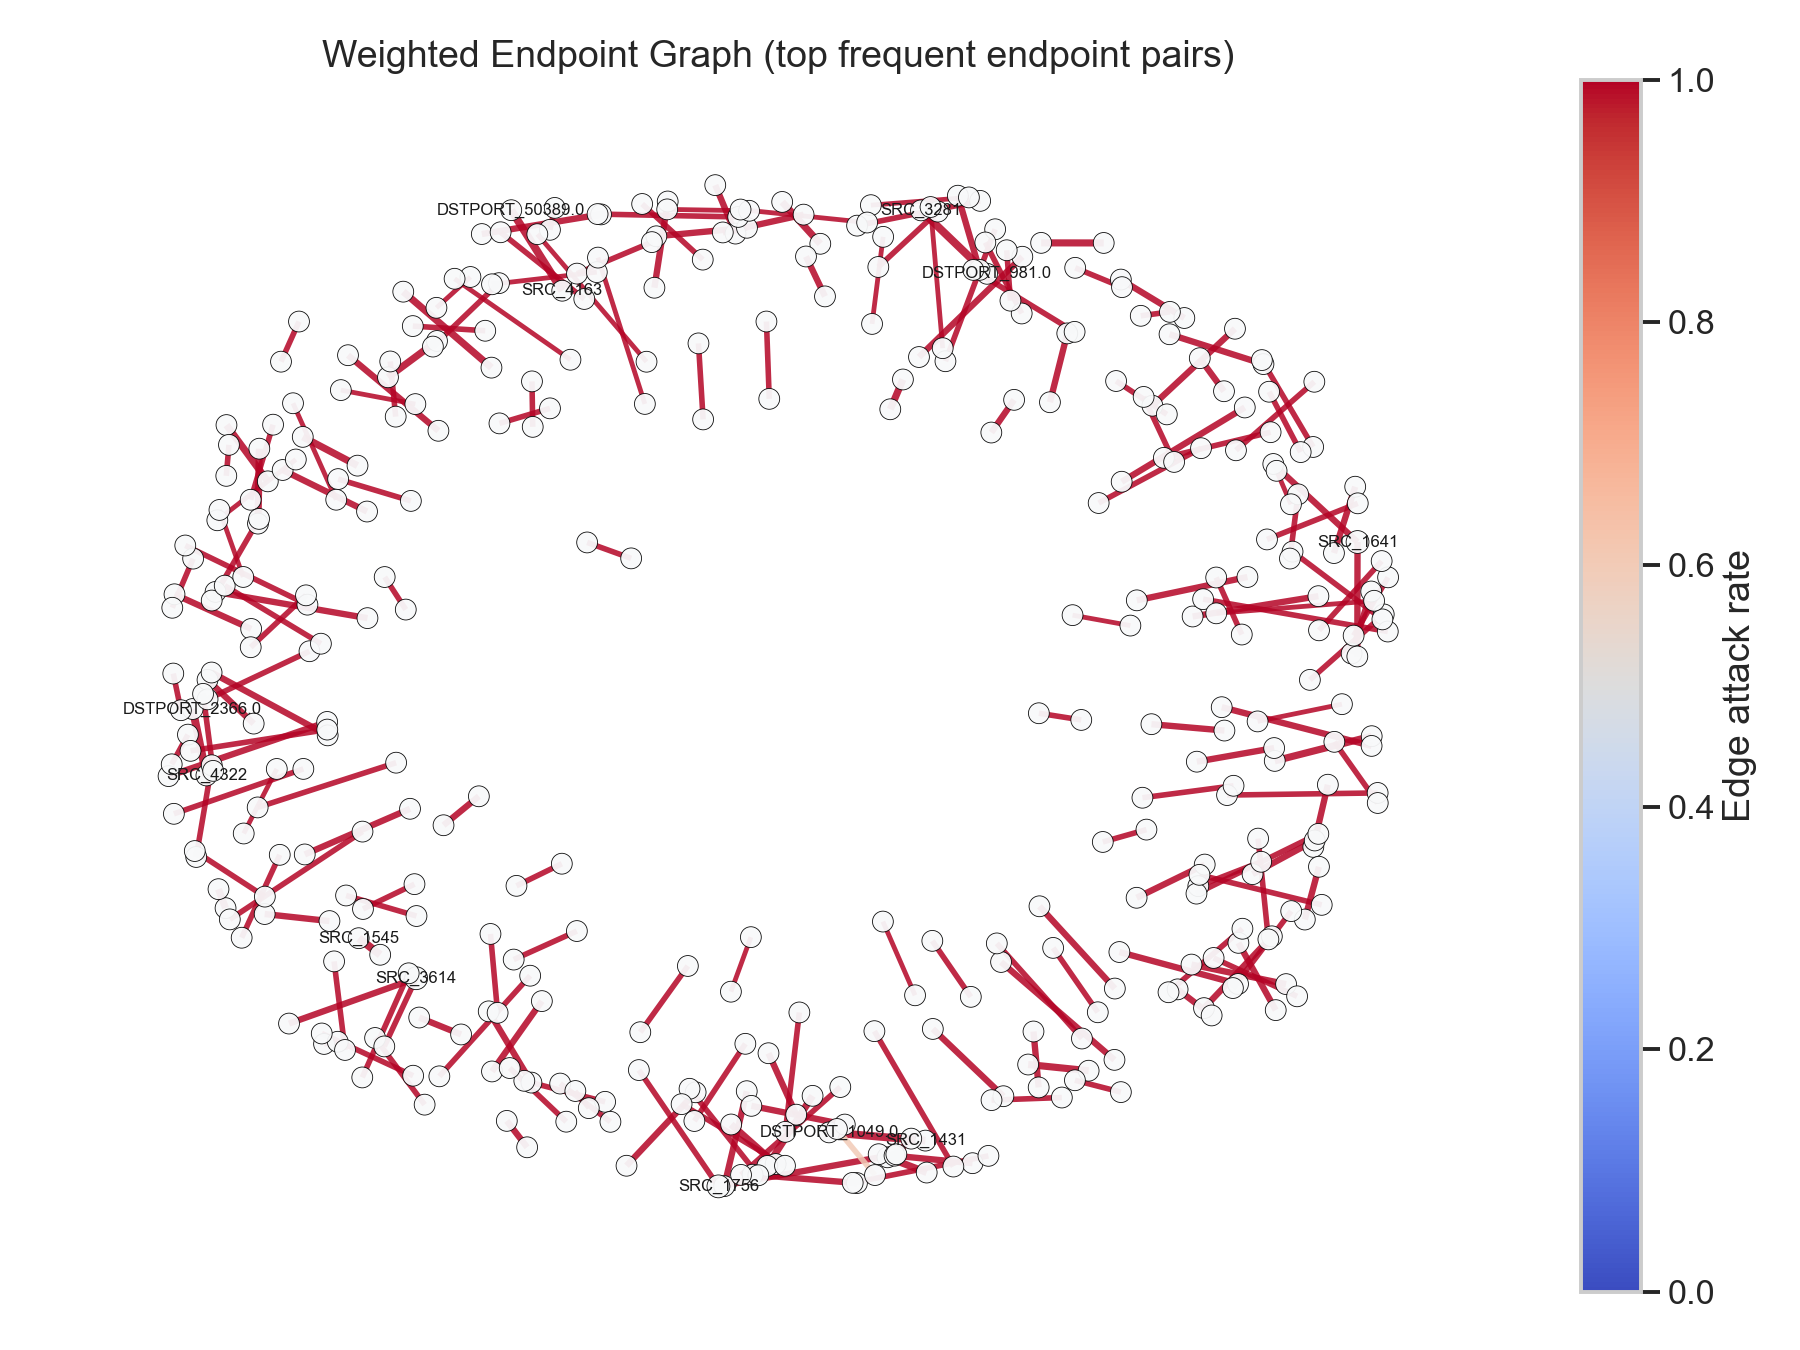
\includegraphics[width=0.32\columnwidth]{constructed_graph_weighted.png}
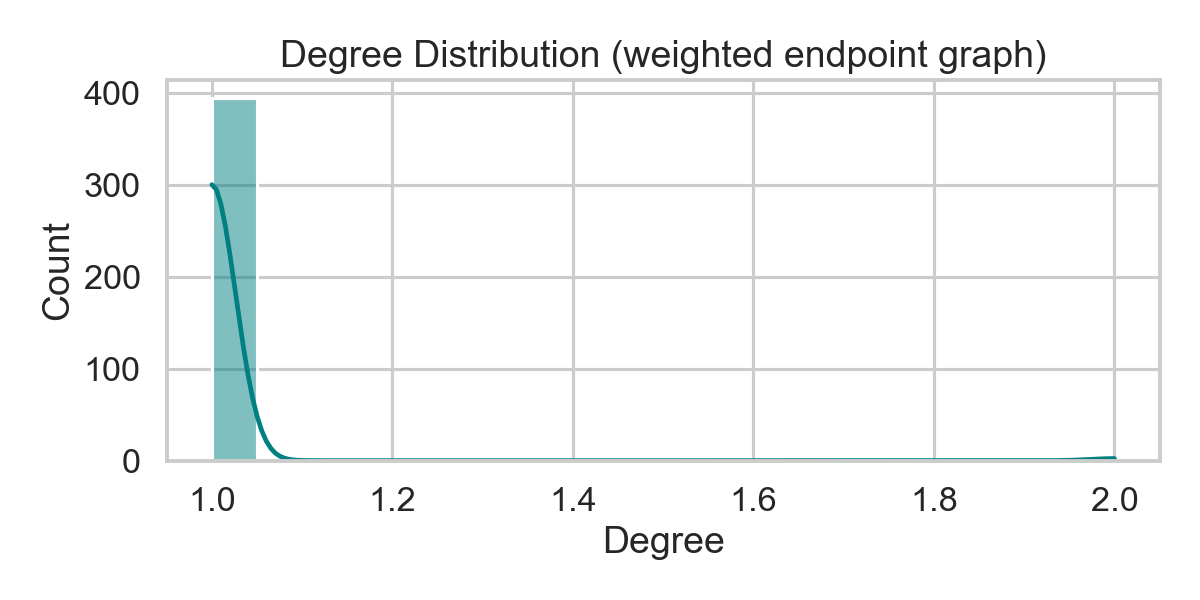
\includegraphics[width=0.32\columnwidth]{constructed_graph_degree_distribution.png}
\caption{Constructed graph examples: snapshot view (left), weighted edge view (center), and degree distribution (right).}
\label{fig:constructed_graphs}
\end{figure}

\begin{figure}[htbp]
\centering
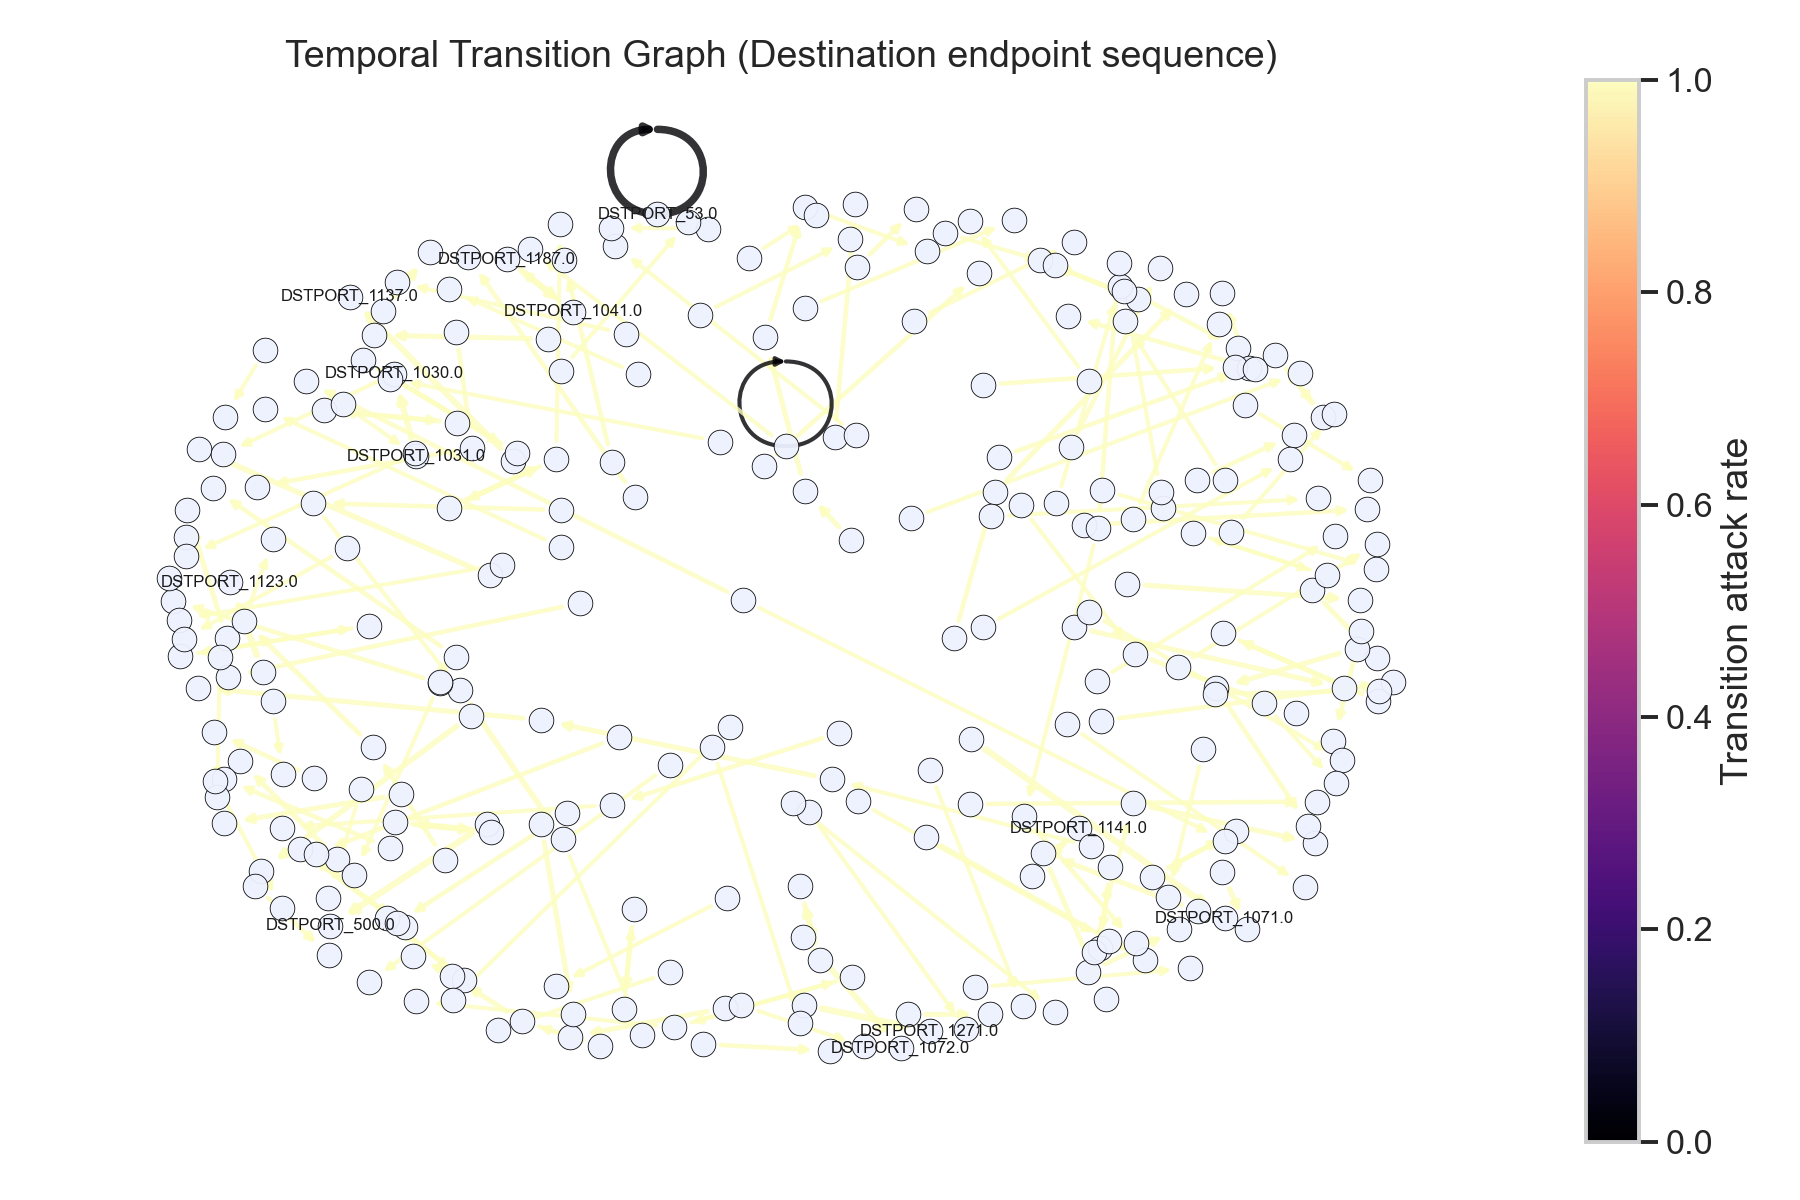
\includegraphics[width=0.95\columnwidth]{constructed_graph_temporal_transitions.png}
\caption{Temporal transitions between consecutive snapshot graphs illustrating evolving connectivity and emerging high-degree nodes during attack phases.}
\label{fig:constructed_transitions}
\end{figure}

\subsection{Realtime Simulation}
Replay simulation across 144 snapshots produced 59 attack-flagged windows, with mean attack probability 0.492 and peak probability 0.9998. The resulting trajectory shows bursty high-confidence periods, which is typical for concentrated attack phases.

In streaming mode, the detector tails an appending flow CSV, assigns new rows into the same fixed snapshot windows, applies the frozen deployment transforms, builds snapshot graphs, and runs inference using a small rolling temporal context buffer. Alerts are emitted per completed window as summary probabilities (mean/max) together with a binary decision based on the saved threshold.

\begin{figure}[htbp]
\centerline{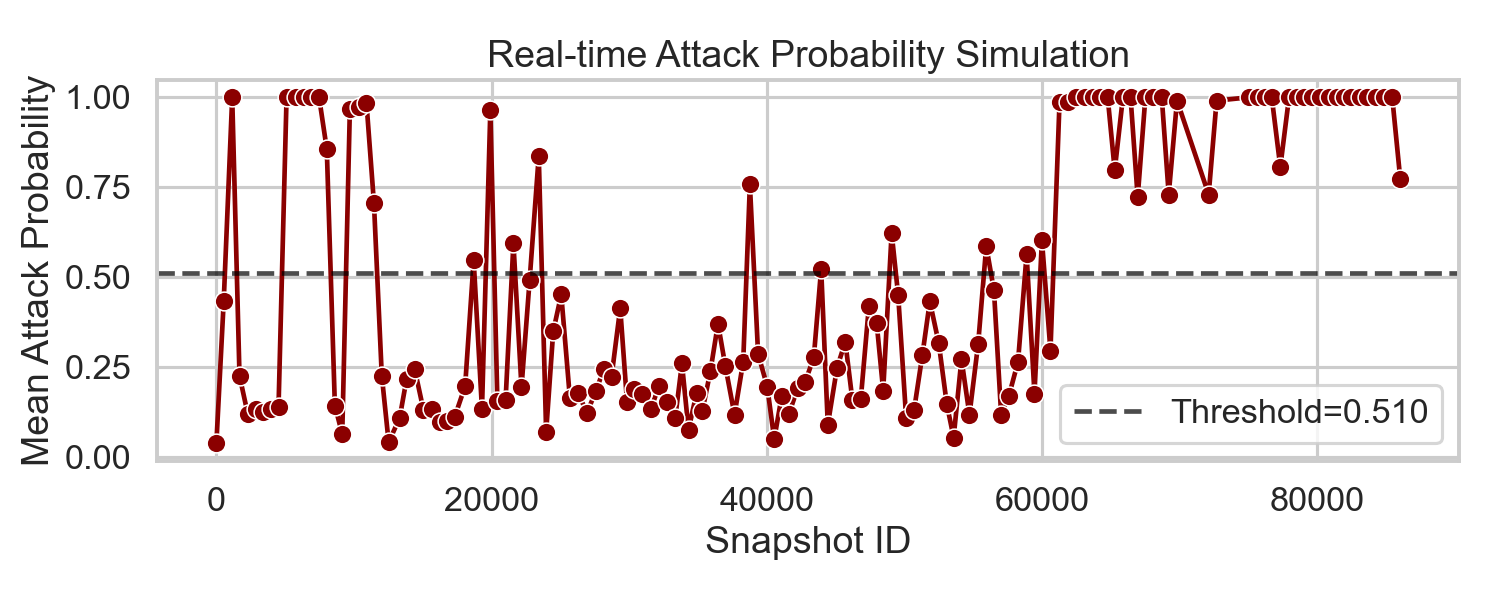
\includegraphics[width=0.95\columnwidth]{realtime_attack_probability.png}}
\caption{Snapshot-level attack probability during realtime simulation replay.}
\label{fig:realtime}
\end{figure}

% "Additional evaluation artifacts" section removed per request.

\section{Limitations and Threats to Validity}
Current repository artifacts do not yet include complete multi-seed significance outputs for the latest upgraded model revision, so statistical claims should be interpreted as point estimates from available runs. In addition, deployment realism still depends on live schema stability (feature columns and timestamp quality) and on periodic recalibration under drift.

\section{Conclusion}
This project demonstrates a practical path from temporal graph learning to explainable near-real-time cyberattack detection. The upgraded TemporalGNN model delivers strong ROC-AUC and robust F1 under low FAR constraints, while explanation artifacts improve analyst transparency. Next steps include full multi-seed significance for the upgraded configuration, online drift monitoring, and closed-loop SOC feedback for threshold adaptation.

\bibliographystyle{IEEEtran}
\bibliography{references}

\end{document}
